\documentclass{article}
\usepackage[utf8]{inputenc}


\usepackage{tikz}
\usepackage{pgfplots,pgfplotstable}\pgfplotsset{compat=1.9}
\usetikzlibrary{pgfplots.groupplots}

\usetikzlibrary{external}
\tikzexternalize[prefix=tikz/]
\usetikzlibrary{patterns,fadings}
\title{Results}
\author{Tony}
\date{February 2019}

\begin{document}

\maketitle

\pgfplotstableread[col sep = comma]{device_name_vs_num_users.csv}\SecurityDeviceStat

\makeatletter
\pgfplotsset{
    /pgfplots/flexible xticklabels from table/.code n args={3}{%
        \pgfplotstableread[#3]{#1}\coordinate@table
        \pgfplotstablegetcolumn{#2}\of{\coordinate@table}\to\pgfplots@xticklabels
        \let\pgfplots@xticklabel=\pgfplots@user@ticklabel@list@x
    }
}
\makeatother

\section{Device Name vs Number of Users }

\begin{figure}
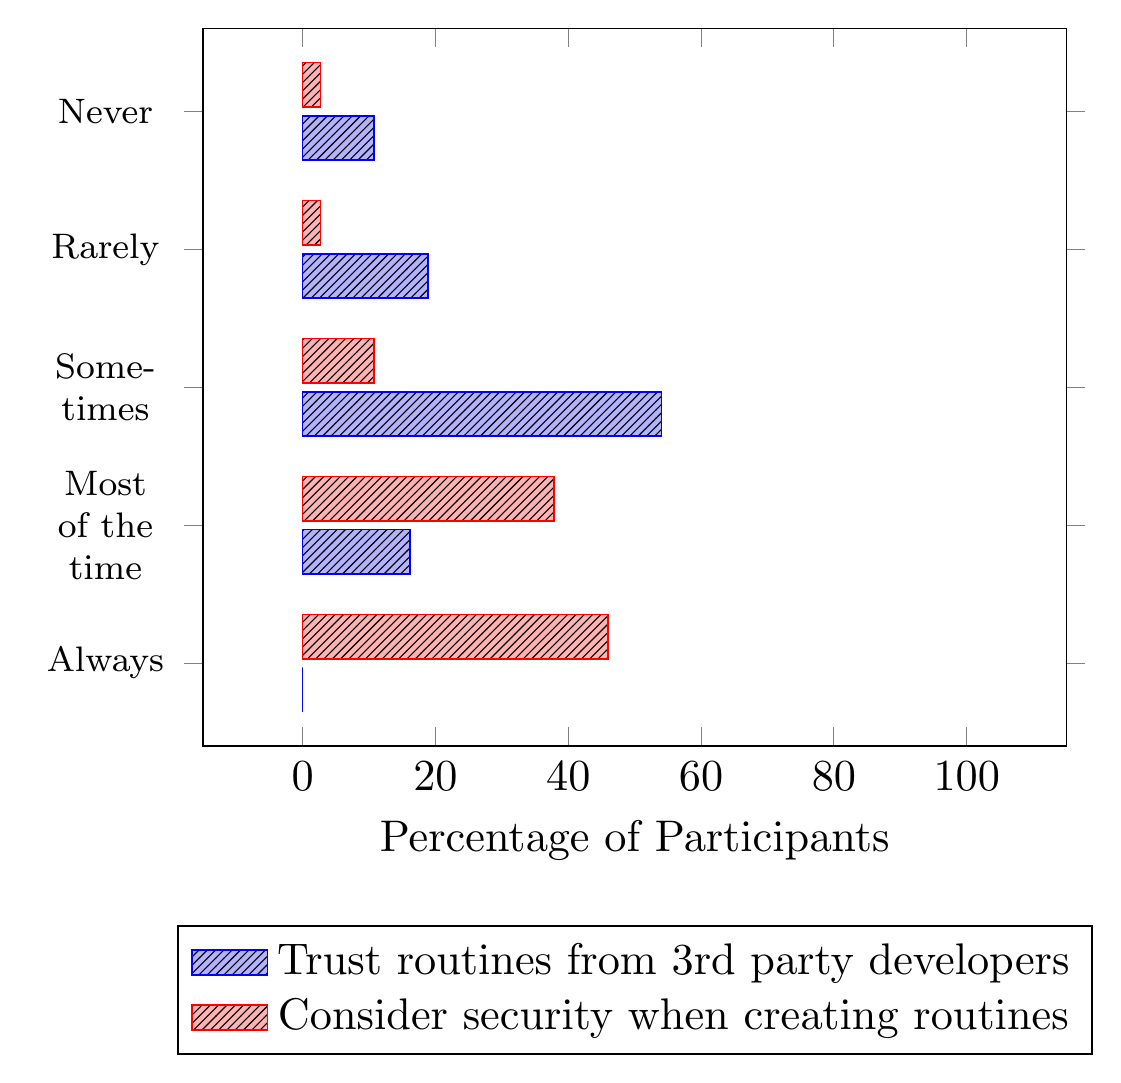
\begin{tikzpicture}[scale=1.6,transform shape]
\begin{axis}[
xbar,
xmax=100,
enlargelimits=0.15,
legend style={at={(0.5,-0.25)},anchor=north},
xlabel={Percentage of Participants},
symbolic y coords={Always,Most of the time,Some-times,Rarely,Never},
xtick={0,20,40,60,80,100},
yticklabel style={text width=1.0cm,
font=\footnotesize,
label style={font=\large},
align=center
},
area legend,		
]
%3d party
\addplot[draw=blue,fill=blue!30!white,postaction={pattern=north east lines}]
coordinates{(54.05,Some-times) (18.91,Rarely) (0,Always)  (16.21,Most of the time) (10.81,Never) };
\addlegendentry{Trust routines from 3rd party developers}
% %Consider security
\addplot[draw=red,fill=red!30!white,postaction={pattern=north east lines}]
coordinates {(10.81,Some-times) (2.70,Rarely) (45.94,Always)  (37.83,Most of the time) (2.70,Never)
};

% \legend{Consider Security \\when creating routines,Trust Routines by 3rd party developers}
\addlegendentry{Consider security when creating routines}

\end{axis}
\end{tikzpicture}
\caption{Figure 10}
\label{GedaechtnisBilder}
\end{figure}


% \begin{tikzpicture}
%     \begin{axis}
%         \addplot table [col sep=comma,x=y, y=x] {\pgfplotstableread{
% x y
% 0 0
% 2 2
% 1 3
% }}
%    \end{axis}
% \end{tikzpicture}

% \begin{figure}
% \begin{tikzpicture}[scale=1.6,transform shape]
% \begin{axis}[
% xbar,
% xmax=100,
% enlargelimits=0.15,
% legend style={at={(0.5,-0.25)},anchor=north},
% xlabel={Percentage of Participants},
% symbolic y coords={Always,Most of the time,Some-times, Rarely,Never},
% ytick=data,
% xtick={0,20,40,60,80,100},
% yticklabel style={text width=1.0cm,
% font=\footnotesize,
% label style={font=\large},
% align=center
% },
% ]
% %3d party
% \addplot table[col sep=comma,x=1,y=0]{
% Some-times,54.05
% Rarely,18.91 
% Always,0
% Most of the time,16.21 
% Never,10.81
% };
% \addlegendentry{Trust routines from 3rd party developers}
% %Consider security
% % \addplot[red,fill=red!30!white,x index=1,y index=0] plot table[ignore chars={(,)},col sep=comma,x index=1,y index=0]
% % {(Some-times,10.81) (Rarely,2.70) (Always,45.94)  (Most of the time,37.83) (Never,2.70)
% % };
% % %\legend{Consider Security \\when creating routines,Trust Routines by 3rd party developers}
% % \addlegendentry{Consider security when creating routines}

% \end{axis}
% \end{tikzpicture}
% \caption{Unterschrift}
% \label{GedaechtnisBilder}
% \end{figure}


\end{document}
